% % % % % % % % % % % % % % % % % % % % % % % % % % % % % % % % % %
%  Devolutiva — Fase 1: Imersão
%  Disciplina: Design Thinking (DE_233) — ETE Cícero Dias
%  Profa. Samara Silva  ·  Recife, 28 de junho de 2026
% % % % % % % % % % % % % % % % % % % % % % % % % % % % % % % % % %

\documentclass[
  sigconf,
  nonacm, % Remove o rodapé da ACM
  language=portuguese
]{acmart}

% ── Desliga rodapé ACM ──────────────────────────────────────
\settopmatter{printacmref=false}
\setcopyright{none}
\acmYear{2026}
\let\balance\relax

% ── Mata a página temporária da ACM (compilação única via API) ──
\makeatletter
\def\acm@addtemp@page{}
\makeatother

% ── Pacotes ─────────────────────────────────────────────────
\usepackage[portuguese]{babel}
\usepackage{microtype}
\usepackage{booktabs}
\usepackage{tabularx}
\usepackage{array}
\usepackage{colortbl}
\usepackage[dvipsnames,table]{xcolor}
\usepackage[inline]{enumitem}
\usepackage{graphicx}
\usepackage{adjustbox}
\usepackage{fancyhdr}
\usepackage{eso-pic} % Para a capa preencher toda a página sem gerar páginas em branco

% ── Ajuste contra quebras de texto ruins (Textos Cortados) ──
\tolerance=1000
\emergencystretch=1.5em

% ── Cores ───────────────────────────────────────────────────
\definecolor{cgood}{HTML}{1E6B3A}
\definecolor{cwarn}{HTML}{8B4500}
\definecolor{cred}{HTML}{C0392B}
\definecolor{cmuted}{HTML}{666666}
\definecolor{crow}{HTML}{F2EFEB}

% ── Colunas customizadas para tabela ────────────────────────
\newcolumntype{L}[1]{>{\raggedright\arraybackslash}p{#1}}
\newcolumntype{C}[1]{>{\centering\arraybackslash}p{#1}}

% ── Comando nota destacada ───────────────────────────────────
\newcommand{\notadestaque}[2]{%
  \noindent\textbf{Nota:}\enspace%
  {\large\bfseries\color{cred}#1\,/\,#2\,pts}%
}

% ── Comando label de status ──────────────────────────────────
\newcommand{\statusok}[1]{{\small\bfseries\color{cgood}#1}}
\newcommand{\statuswarn}[1]{{\small\bfseries\color{cwarn}#1}}

% ── Renomeações PT-BR ────────────────────────────────────────
\AtBeginDocument{%
  \renewcommand{\abstractname}{Resumo}
  \renewcommand{\figurename}{Figura}
  \renewcommand{\tablename}{Tabela}
}

% ────────────────────────────────────────────────────────────
\begin{document}

% ── CAPA ────────────────────────────────────────────────────
\thispagestyle{empty}
\AddToShipoutPictureBG*{%
  \AtPageLowerLeft{%
    \IfFileExists{capa.png}{%
      
\includegraphics[width=\paperwidth,height=\paperheight]{capa.png}%
    }{%
      \IfFileExists{../../capa.png}{%
        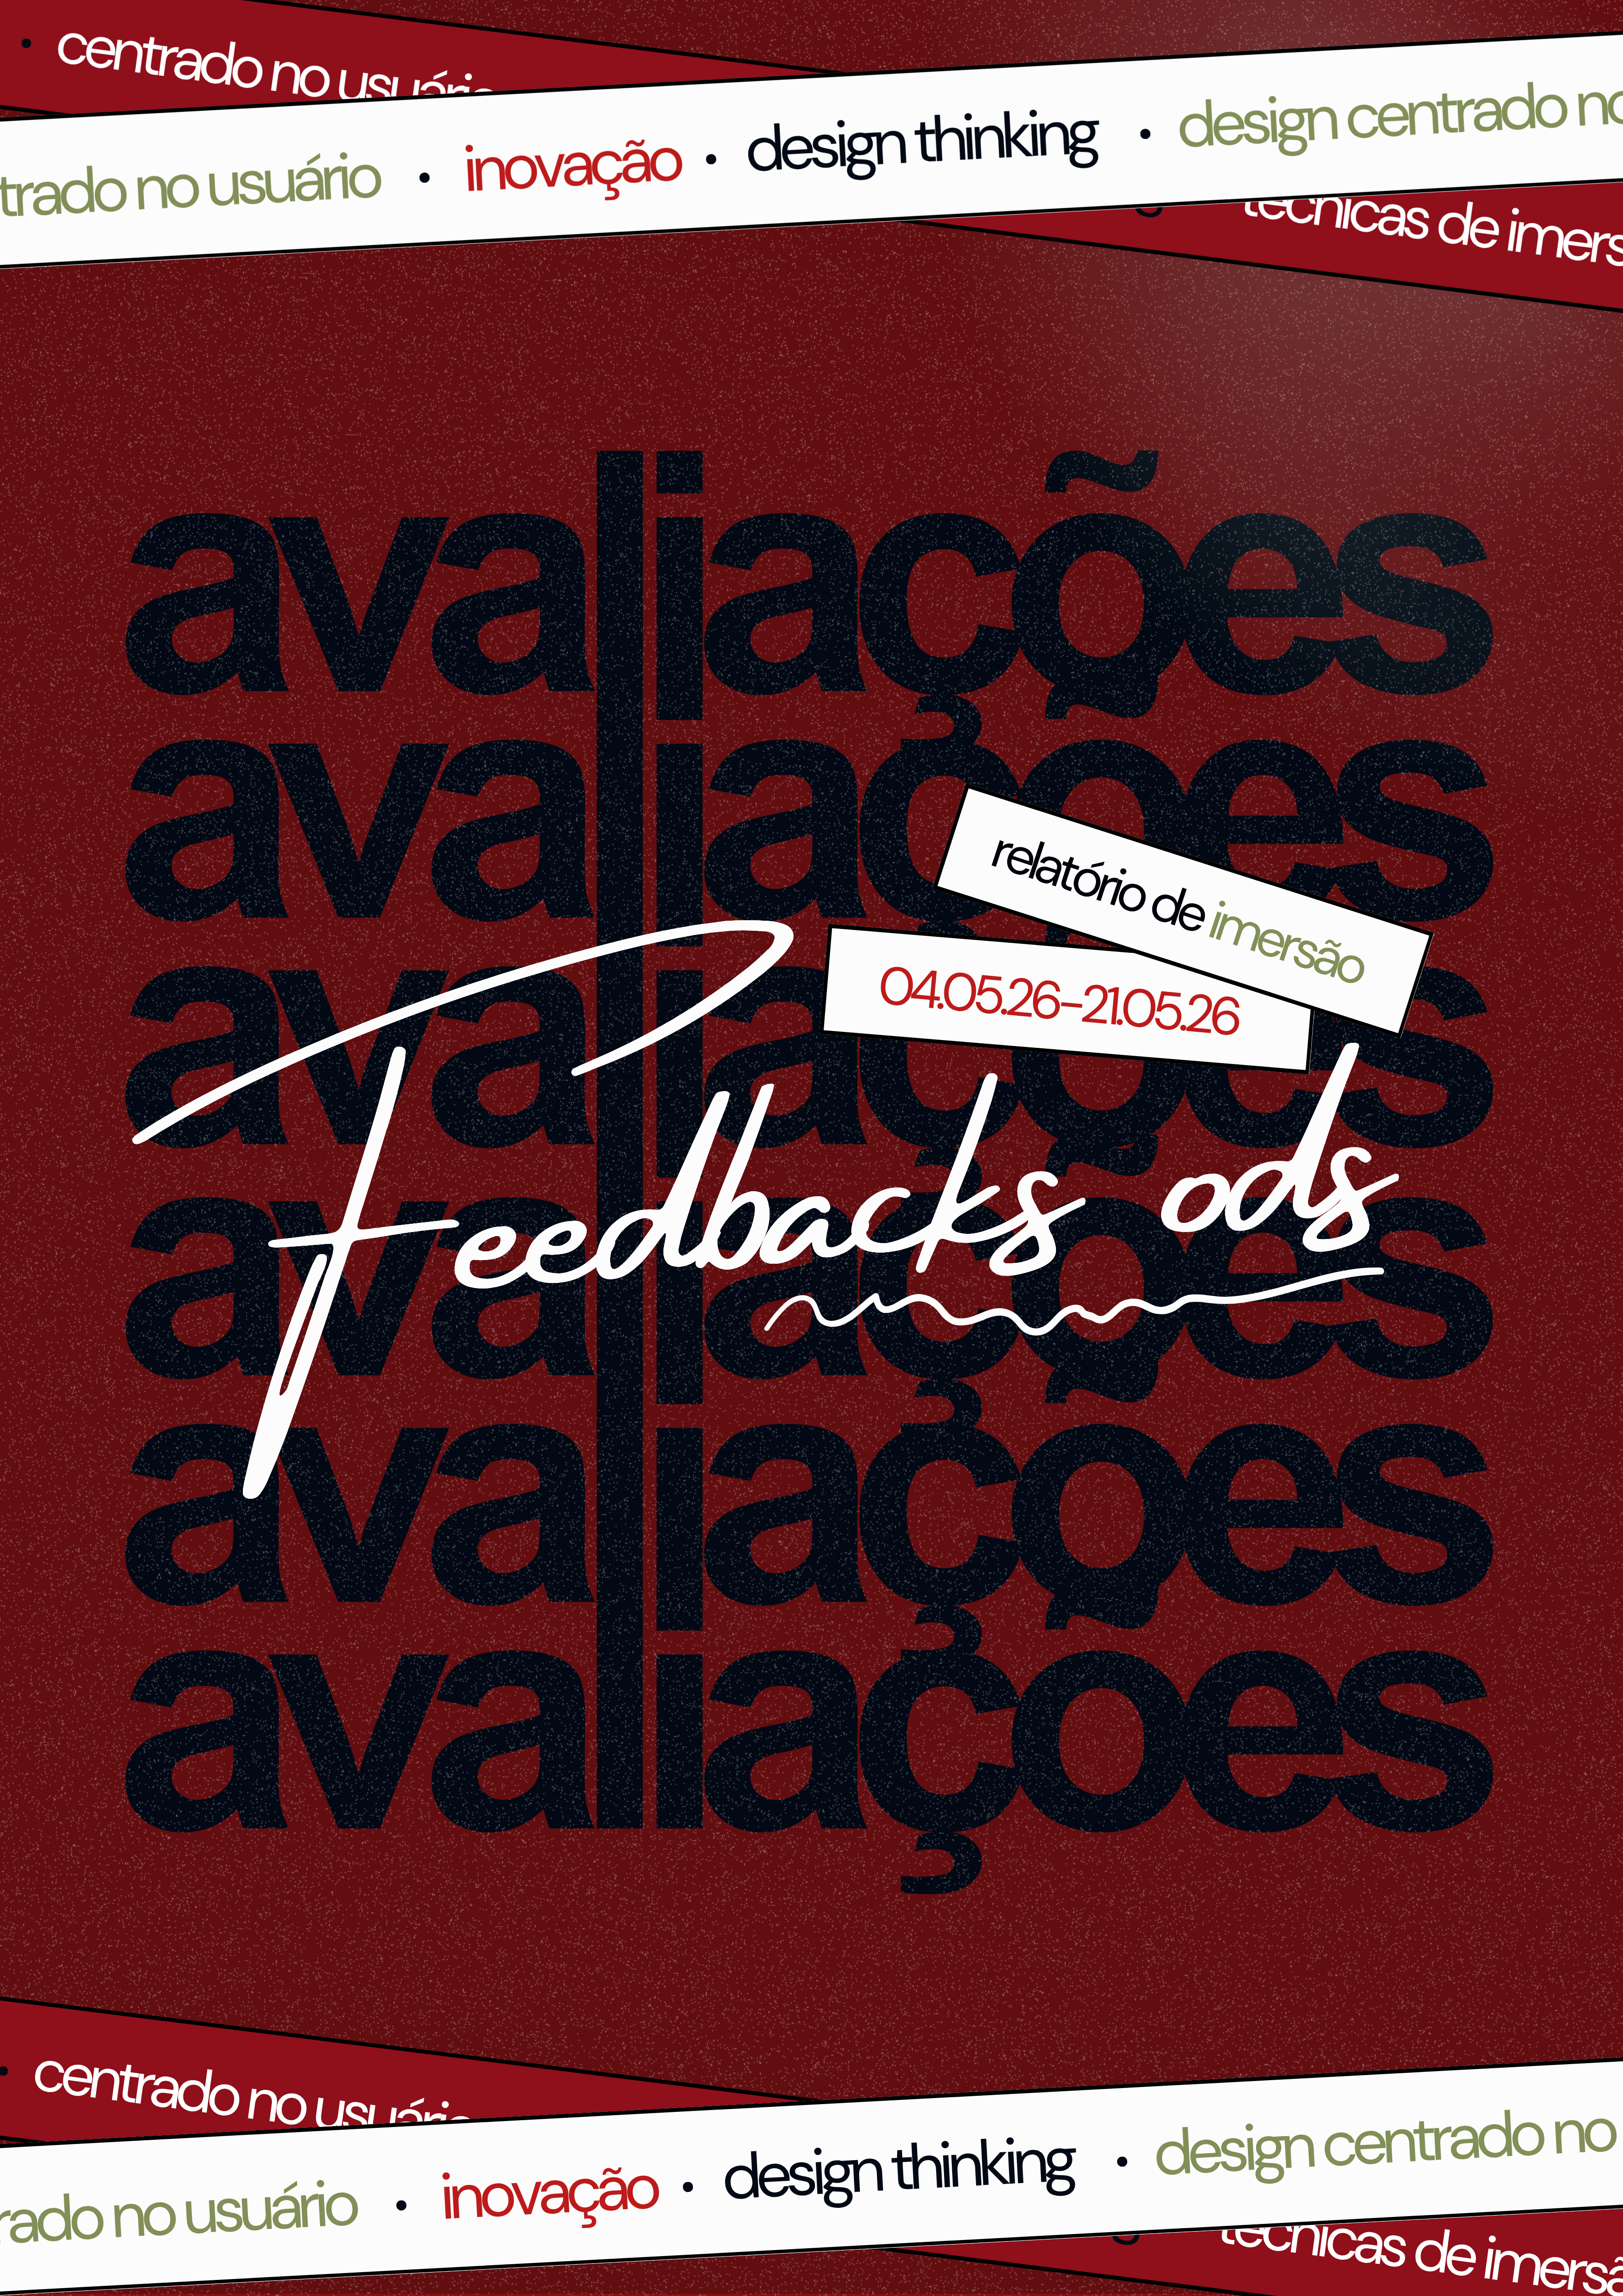
\includegraphics[width=\paperwidth,height=\paperheight]{../../capa.png}%
      }{%
        \parbox[b][\paperheight]{\paperwidth}{%
          \vspace*{10cm}\begin{center}{\large\color{gray}[capa.png não encontrada]}\end{center}%
        }%
      }%
    }%
  }%
}
\mbox{} % Caixa vazia para garantir que a página da capa seja gerada e preenchida
\clearpage

% ── CONFIGURAÇÃO DE PÁGINA PÓS-CAPA ─────────────────────────
\setcounter{page}{1}
\pagestyle{fancy}
\fancyhf{}
\renewcommand{\headrulewidth}{0pt}
\fancyfoot[C]{\thepage}
\setlength{\headsep}{0.8cm} % Distancia o cabeçalho do conteúdo das colunas

% ── METADADOS ────────────────────────────────────────────────
\title{Feedback Avaliativo de Projeto: Design Thinking --- Avaliação Completa}

\author{Profa.\ Samara Silva}
\authornote{Grupo: \textbf{Grupo 01 - Fome Zero} \textperiodcentered\ Per\'{i}odo: 22 de maio de 2026 \textperiodcentered\ Avaliado em: 28 de junho de 2026.}
\email{samarasilvia.educa@gmail.com}
\affiliation{%
  \institution{ETE C\'{i}cero Dias}
  \department{M\'{o}dulo 1 --- Turma A · 2026.1}
  \city{Recife}
  \state{Pernambuco}
  \country{Brasil}
}

\author{Grupo 01 - Fome Zero}
\affiliation{%
  \institution{ETE C\'{i}cero Dias}
  \department{Turma --- Turma A · 2026.1}
  \city{Recife}
  \state{Pernambuco}
  \country{Brasil}
}
\maketitle

\vspace{1em}
\section{Avaliação — Design Thinking}

\notadestaque{10,35}{11,00}

A seguir o detalhamento por fase da disciplina.

\subsection{Fase 1 — Imersão}

\notadestaque{2,35}{3,00}

\subsubsection*{Resumo dos Critérios}

\rowcolors{2}{crow}{white}
\begin{tabular}{@{} L{2.6cm} C{2.5cm} C{1.1cm} C{1.1cm} @{}}
\toprule
\textbf{Critério} & \textbf{Status} & \textbf{Nota} & \textbf{Máx.} \\
\midrule
Pesquisa Desk & \statusok{Completo} & \textbf{0,50} & 0,50 \\
Matriz de Alinhamento & \statusok{Completo} & \textbf{0,50} & 0,50 \\
Matriz CSD \& Perguntas de pesquisa & \statusok{Completo} & \textbf{0,50} & 0,50 \\
Pesquisa Primária & \statuswarn{Completo c/ ressalvas} & \textbf{0,85} & 1,50 \\
\midrule
\textbf{Total} & & \textbf{\color{cred}2,35} & \textbf{3,00} \\
\bottomrule
\end{tabular}

\subsubsection*{Comentários}

\subsection{Pesquisa Desk}

\noindent\statusok{0,50\,/\,0,50 pts · Completo}

\begin{itemize}[leftmargin=14pt,itemsep=1pt,topsep=3pt,parsep=0pt]
  \item[\textcolor{cgood}{$\checkmark$}] {\small\textcolor{cgood}{Dados secundários relevantes e atuais sobre o ODS escolhido}}
  \item[\textcolor{cgood}{$\checkmark$}] {\small\textcolor{cgood}{Fontes confiáveis: ONU, IBGE, artigos acadêmicos ou jornalísticos}}
  \item[\textcolor{cgood}{$\checkmark$}] {\small\textcolor{cgood}{Contextualiza o problema com base factual}}
  \item[\textcolor{cgood}{$\checkmark$}] {\small\textcolor{cgood}{Conexão clara entre os dados e o problema}}
  \item[\textcolor{cgood}{$\checkmark$}] {\small\textcolor{cgood}{Coerência entre a CSD e o que foi pesquisado}}
  \item[\textcolor{cgood}{$\checkmark$}] {\small\textcolor{cgood}{Mínimo de 5 referências/links, esperado 8, ideal de 15 para cima}}
\end{itemize}

O grupo está de parabéns pela qualidade da Desk Research! A escolha das fontes demonstra muita maturidade. Vocês buscaram referências com altíssima credibilidade (FAO, IBGE, EMBRAPA, MAPA) e dados extremamente atualizados, o que traz um embasamento fantástico para justificar a importância do projeto. Senti falta de dados diferentes como artigos ou algo de teor acadêmico, mas não tira o mérito do trabalho.

\textit{\textbf{Seção presente no relatório}}

A redação desta seção está excelente! O texto é extremamente claro, bem fundamentado e utiliza uma linguagem técnica e acadêmica perfeitamente adequada ao rigor exigido pelo projeto. A forma como vocês dividiram as frentes estratégicas (Análise Documental, Quantitativa e Levantamento Bibliográfico) demonstra muita organização e maturidade metodológica.

Outro ponto fortíssimo do trabalho foi a consolidação das inferências no final do texto. Extrair os dados da pesquisa teórica e estruturá-los de forma quantitativa (Dado 1 a Dado 6) para a construção de gráficos foi uma excelente decisão. Isso não apenas facilita a leitura e a visualização do problema, mas também comprova a capacidade analítica da equipe em transformar textos densos em informações acionáveis que justificam a criação do aplicativo.

Ótimo trabalho de síntese e argumentação! Parabéns, fiquei muito feliz com o trabalho de vocês.

\subsection{Matriz de Alinhamento}

\noindent\statusok{0,50\,/\,0,50 pts · Completo}

\begin{itemize}[leftmargin=14pt,itemsep=1pt,topsep=3pt,parsep=0pt]
  \item[\textcolor{cgood}{$\checkmark$}] {\small\textcolor{cgood}{Identifica claramente quem é afetado pelo problema}}
  \item[\textcolor{cgood}{$\checkmark$}] {\small\textcolor{cgood}{Define o que o grupo pretende descobrir durante a imersão}}
  \item[\textcolor{cgood}{$\checkmark$}] {\small\textcolor{cgood}{As técnicas de imersão escolhidas são coerentes com os objetivos da pesquisa}}
  \item[\textcolor{cgood}{$\checkmark$}] {\small\textcolor{cgood}{Delimita adequadamente o que está dentro do escopo do projeto}}
  \item[\textcolor{cgood}{$\checkmark$}] {\small\textcolor{cgood}{Delimita adequadamente o que está fora do escopo do projeto}}
  \item[\textcolor{cgood}{$\checkmark$}] {\small\textcolor{cgood}{Apresenta uma hipótese inicial de solução relacionada ao problema investigado}}
  \item[\textcolor{cgood}{$\checkmark$}] {\small\textcolor{cgood}{Os resultados esperados da imersão são claros e coerentes com os objetivos da pesquisa}}
  \item[\textcolor{cgood}{$\checkmark$}] {\small\textcolor{cgood}{Há coerência entre os diferentes campos da matriz (problema, público, escopo, pesquisa e solução)}}
  \item[\textcolor{cgood}{$\checkmark$}] {\small\textcolor{cgood}{Preenchida com respostas, impressões ou perguntas reais do grupo sobre o problema}}
  \item[\textcolor{cgood}{$\checkmark$}] {\small\textcolor{cgood}{Linguagem clara e coerente, facilitando a compreensão das intenções do grupo}}
  \item[\textcolor{cgood}{$\checkmark$}] {\small\textcolor{cgood}{Serviu de base para planejar a pesquisa primária}}
\end{itemize}

Nada a declarar. Está tudo de acordo com o esperado!

\subsection{Matriz CSD \& Perguntas de pesquisa}

\noindent\statusok{0,50\,/\,0,50 pts · Completo}

\begin{itemize}[leftmargin=14pt,itemsep=1pt,topsep=3pt,parsep=0pt]
  \item[\textcolor{cgood}{$\checkmark$}] {\small\textcolor{cgood}{Os três quadrantes preenchidos: Certezas, Suposições, Dúvidas}}
  \item[\textcolor{cgood}{$\checkmark$}] {\small\textcolor{cgood}{Reflete o que o grupo sabe e precisa descobrir sobre o problema e seu contexto}}
  \item[\textcolor{cgood}{$\checkmark$}] {\small\textcolor{cgood}{Conteúdo específico do projeto — não genérico}}
  \item[\textcolor{cgood}{$\checkmark$}] {\small\textcolor{cgood}{Revela pensamento crítico}}
  \item[\textcolor{cgood}{$\checkmark$}] {\small\textcolor{cgood}{O quadrante de CERTEZAS expõe informações comprovadas ou confirmadas sobre o problema}}
  \item[\textcolor{cgood}{$\checkmark$}] {\small\textcolor{cgood}{Os itens do quadrante de CERTEZA estão relacionados diretamente ao contexto e ao público afetado}}
  \item[\textcolor{cgood}{$\checkmark$}] {\small\textcolor{cgood}{O quadrante de SUPOSIÇÕES expõe Informações que o grupo acha que são verdadeiras, mas ainda não comprovou}}
  \item[\textcolor{cgood}{$\checkmark$}] {\small\textcolor{cgood}{Os itens do quadrante de SUPOSIÇÃO demonstram reflexão sobre possíveis causas, comportamentos ou necessidades}}
  \item[\textcolor{cgood}{$\checkmark$}] {\small\textcolor{cgood}{O quadrante de DÚVIDAS expõem perguntas que o grupo precisa responder na pesquisa ou imersão como um todo}}
  \item[\textcolor{cgood}{$\checkmark$}] {\small\textcolor{cgood}{Os itens do quadrante de DÚVIDAS representam lacunas reais de conhecimento}}
  \item[\textcolor{cgood}{$\checkmark$}] {\small\textcolor{cgood}{O conteúdo da matriz está focado no problema investigado e não apenas no tema ou na ODS}}
  \item[\textcolor{cgood}{$\checkmark$}] {\small\textcolor{cgood}{Perguntas de Pesquisas formuladas como objetivos que norteiam o projeto geral}}
  \item[$\square$] {\small\textcolor{cmuted}{Deve se ter um mínimo de 5 itens no quadrante de certezas, suposições e dúvidas}}
\end{itemize}

A equipe demonstrou um bom entendimento na construção da Matriz CSD, que é um excelente ponto de partida. A coluna de 'Dúvidas' está muito bem construída e contém pontos altamente estratégicos. Eu particularmente adorei que abrangeram vários escopos desde algo financeiro até logístico.

No entanto, há um desvio metodológico importante na etapa de planejamento das perguntas de pesquisa que precisa ser corrigido: \textbf{houve uma sobreposição entre as Perguntas de Pesquisa e o Roteiro/Formulário do usuário. }Para o rigor acadêmico e prático do Design de Serviços/Produtos, é fundamental distinguir estas três camadas:

\begin{itemize}[leftmargin=14pt,itemsep=2pt,topsep=4pt]
  \item \textbf{Dúvidas (Matriz CSD):} Representam as incertezas internas do grupo. É o levantamento bruto do que a equipe não sabe. ex:\textit{"Os estudantes preferem estudar pelo celular ou pelo notebook?"}
  \item \textit{"Eles ainda têm o costume de usar agenda de papel?"}
  \item \textit{"Quanto tempo eles conseguem focar antes de pegar o celular?"}
\end{itemize}

\begin{itemize}[leftmargin=14pt,itemsep=2pt,topsep=4pt]
  \item \textbf{Perguntas de Pesquisa:} São os objetivos da investigação. Elas guiam o \textit{projeto} e a \textit{equipe}, sintetizando as dúvidas e suposições da CSD em grandes eixos investigativos. \textbf{Essas perguntas não devem ser feitas diretamente ao usuário. }ex:\textit{"Quais são os principais métodos e ferramentas de organização utilizados por universitários hoje, e quais são os maiores gatilhos comportamentais de distração durante o estudo?"}
\end{itemize}

\begin{itemize}[leftmargin=14pt,itemsep=2pt,topsep=4pt]
  \item \textbf{Roteiro/Formulário de Pesquisa:} É o instrumento de coleta. Aqui, as perguntas de pesquisa são traduzidas para a linguagem do usuário, de forma conversacional e empática, para evitar vieses. ex:\textit{"Você poderia me contar como costuma se organizar quando tem uma semana cheia de provas?"}
  \item \textit{"Lembre da última vez que você sentou para estudar e acabou perdendo o foco. Como foi isso? O que acabou tirando a sua atenção?"}
\end{itemize}

\textbf{O impacto desse erro:} Em vez de definirem os eixos estratégicos que o projeto precisa investigar, a equipe inseriu as perguntas de interação direta com o usuário no lugar das Perguntas de Pesquisa. Ao fazer isso, o projeto perde o seu "norte" analítico.

Por exemplo: a questão que vocês listaram, \textit{"Sobre o descarte de alimentos na sua casa: Quando você prepara refeições, o que costuma fazer com as partes não convencionais dos vegetais e frutas (cascas, talos, folhas e sementes)?"}, é uma excelente pergunta de \textbf{Formulário/Roteiro} para fazer ao usuário. No entanto, a verdadeira \textbf{Pergunta de Pesquisa} (que deveria estar preenchendo essa seção do documento para guiar a equipe) deveria ser algo como: \textbf{"Quais são os hábitos atuais de descarte e o nível de aproveitamento integral dos alimentos na rotina doméstica do nosso público?"}

\textbf{Ação necessária:} Revisar o instrumento de pesquisa. Desdobrem as Perguntas de Pesquisa atuais em perguntas adequadas e táticas.

\subsection{Pesquisa Primária}

\noindent\statuswarn{0,85\,/\,1,50 pts · Completo c/ ressalvas}

\textit{\textbf{Seção presente no relatório}}

O texto que descreve os resultados da pesquisa está excelente. A redação é clara, objetiva e traz inferências muito ricas. A forma como vocês estruturaram os dados percentuais ao final (Dado Survey 1 ao 5) demonstra uma ótima capacidade de síntese. Vocês conseguiram cruzar as respostas para comprovar a viabilidade e a aceitação do aplicativo, o que atende perfeitamente ao objetivo desta etapa. Parabéns pela estruturação!

\textit{\textbf{InStrumento de coleta (Google forms)}}

Embora a estrutura básica do formulário esteja correta e os resultados tenham sido úteis, existem pontos importantes de melhoria para que a pesquisa alcance um rigor metodológico maior em projetos futuros:

\begin{enumerate}[leftmargin=14pt,itemsep=2pt,topsep=4pt]
  \item \textbf{Descrição e Termo de Consentimento:} A introdução do formulário foi muito breve. Faltou especificar que vocês são estudantes do curso de Desenvolvimento de Sistemas da ETE Cícero Dias, detalhar um pouco mais o propósito do projeto e, muito importante em formulários, informar o tempo estimado de resposta (ex: "Esta pesquisa leva apenas 2 minutos").
  \item \textbf{Perfil do Usuário (Dados Demográficos):} O formulário não coleta informações básicas de quem está respondendo. Mesmo sendo anônimo, é fundamental saber a faixa etária, a composição familiar (quantas pessoas moram na casa) e o contexto socioeconômico. Isso permite cruzar dados importantes (ex: "Será que famílias maiores desperdiçam mais?" ou "Qual a idade do público que mais aceita a tecnologia?").
  \item \textbf{Volume e Diversidade de Perguntas:} Um questionário com apenas 5 perguntas limita muito o aprofundamento do tema. O ideal para uma pesquisa desse porte seria entre 10 e 12 perguntas, preferencialmente divididas por seções (Ex: Seção 1 - Perfil; Seção 2 - Hábitos de Consumo; Seção 3 - Relação com Tecnologia).
  \item \textbf{Tipos de Resposta:} Houve uma limitação ao usar apenas perguntas de múltipla escolha (onde só se marca uma opção). Em pesquisas de campo, é enriquecedor incluir perguntas de "caixa de seleção" (onde o usuário pode marcar mais de um motivo) e, principalmente, perguntas abertas (texto curto ou longo) para captar opiniões espontâneas e insights qualitativos que a equipe não havia previsto.
\end{enumerate}

Apesar dessas oportunidades de melhoria no formulário, os dados coletados foram suficientes para embasar a justificativa do projeto nesta etapa. Excelente trabalho de análise!

\subsection{Fase 2 — Definição}

\notadestaque{3,00}{3,00}

\subsubsection*{Resumo dos Critérios}

\rowcolors{2}{crow}{white}
\begin{tabular}{@{} L{2.6cm} C{2.5cm} C{1.1cm} C{1.1cm} @{}}
\toprule
\textbf{Critério} & \textbf{Status} & \textbf{Nota} & \textbf{Máx.} \\
\midrule
Persona com Empatia Real & \statusok{Completo} & \textbf{0,50} & 0,50 \\
Mapa de Empatia como Ferramenta & \statusok{Completo} & \textbf{1,00} & 1,00 \\
Enunciado do Problema & \statusok{Completo} & \textbf{1,00} & 1,00 \\
Jornada do Usuário (ASTOIS) & \statusok{Completo} & \textbf{0,50} & 0,50 \\
\midrule
\textbf{Total} & & \textbf{\color{cred}3,00} & \textbf{3,00} \\
\bottomrule
\end{tabular}

\subsubsection*{Comentários}

\subsection{Persona com Empatia Real}

\noindent\statusok{0,50\,/\,0,50 pts · Completo}

\begin{itemize}[leftmargin=14pt,itemsep=1pt,topsep=3pt,parsep=0pt]
  \item[\textcolor{cgood}{$\checkmark$}] {\small\textcolor{cgood}{Nome próprio que humaniza o arquétipo}}
  \item[\textcolor{cgood}{$\checkmark$}] {\small\textcolor{cgood}{Representação visual coerente (foto/avatar)}}
  \item[\textcolor{cgood}{$\checkmark$}] {\small\textcolor{cgood}{Papel/arquétipo-síntese (o rótulo: ex: "Pequeno Comerciante")}}
  \item[\textcolor{cgood}{$\checkmark$}] {\small\textcolor{cgood}{Dados demográficos (idade, gênero, localização, escolaridade, ocupação, estado civil)}}
  \item[\textcolor{cgood}{$\checkmark$}] {\small\textcolor{cgood}{Contexto/bio que situa a vida da pessoa}}
  \item[\textcolor{cgood}{$\checkmark$}] {\small\textcolor{cgood}{Características de personalidade (traços comportamentais)}}
  \item[\textcolor{cgood}{$\checkmark$}] {\small\textcolor{cgood}{Motivação (o que move)}}
  \item[\textcolor{cgood}{$\checkmark$}] {\small\textcolor{cgood}{Objetivos/metas}}
  \item[\textcolor{cgood}{$\checkmark$}] {\small\textcolor{cgood}{Dores/frustrações}}
  \item[\textcolor{cgood}{$\checkmark$}] {\small\textcolor{cgood}{Citação-síntese que captura a essência}}
  \item[\textcolor{cgood}{$\checkmark$}] {\small\textcolor{cgood}{Ancoragem na imersão — a persona é síntese da pesquisa de campo, não invenção/suposição}}
  \item[\textcolor{cgood}{$\checkmark$}] {\small\textcolor{cgood}{Arquétipo comportamental, não estereótipo ou caricatura}}
  \item[\textcolor{cgood}{$\checkmark$}] {\small\textcolor{cgood}{Coerência interna — motivação → objetivos → dores se sustentam mutuamente}}
  \item[\textcolor{cgood}{$\checkmark$}] {\small\textcolor{cgood}{Conexão com o problema e o ODS do projeto}}
  \item[\textcolor{cgood}{$\checkmark$}] {\small\textcolor{cgood}{Especificidade — detalhes concretos que humanizam vs. genérico ("homem de 40 anos qualquer")}}
  \item[\textcolor{cgood}{$\checkmark$}] {\small\textcolor{cgood}{Define claramente as tarefas críticas que o usuário precisa executar}}
\end{itemize}

\textbf{Impressões antes de ler o relatório}

Com base na leitura da persona e na releitura do primeiro relatório, observa-se que a persona está bem estruturada e coerente com os dados coletados. No entanto, surge uma dúvida em relação à matriz de alinhamento, na qual são citados os possíveis afetados pelo desperdício alimentar — “famílias que enfrentam algum grau de insegurança alimentar e pequenos e médios produtores agrícolas afetados pelo desperdício e renda insuficiente”. Apesar disso, foi construída apenas uma única persona, o que não é devidamente justificado no material.

Nesse sentido, seria importante que o relatório de definição trouxesse uma justificativa mais clara para a escolha de uma única persona. Considerando que os dados predominantes parecem estar mais voltados ao ambiente doméstico e que a solução proposta também segue essa direção, poderia ser coerente explicar a priorização desse recorte.

\textbf{VISÃO GERAL DA PERSONA}

A persona Juliana foi bem construída de forma geral, mas alguns elementos importantes poderiam ser melhor detalhados. Entre eles, a ausência de informações como gênero e traços de personalidade, que ajudam a compor uma compreensão mais completa do perfil. Embora algumas dessas características possam parecer implícitas, sua explicitação contribui para maior clareza analítica.

\textit{\textbf{Objetivos e Motivações da Persona}}

Outro ponto é a ausência de objetivos bem definidos. Embora existam motivações descritas, elas não se confundem com objetivos. Motivações estão relacionadas às necessidades e contextos que impulsionam a persona, enquanto objetivos representam resultados práticos que ela busca alcançar.

Por exemplo, no caso de Adalberto trabalhado em sala, sua motivação estava relacionada à necessidade de manter seu comércio funcionando diante dos alagamentos, enquanto seus objetivos eram mais concretos, como receber alertas de chuva com antecedência, reduzir perdas financeiras, estabelecer um canal de comunicação com a prefeitura e retomar rapidamente as atividades após eventos climáticos.

Nesse sentido, parte do que foi descrito como motivação na persona Juliana poderia ser melhor reestruturado, diferenciando o que é contexto de vida, necessidade central e objetivos. Situações mais estruturais, como dificuldade em realizar refeições, podem ser compreendidas como parte das motivações ou do contexto de vida, enquanto os objetivos deveriam refletir ações ou resultados desejados de forma mais direta.

Observa-se uma possível sobreposição entre os campos de “Motivações”, “Contexto de vida” e “Necessidade central”. Algumas informações presentes nas motivações possuem característica de objetivos mais práticos, enquanto parte do contexto de vida poderia contribuir melhor como base explicativa dessas motivações. Uma reorganização desses elementos poderia deixar a hierarquia da persona mais clara, distinguindo melhor o que é contexto, necessidade e objetivo.

\textit{\textbf{Papel/Arquétipo da Persona}}

Outro ponto de reflexão é a escolha da profissão da persona, no caso “auxiliar administrativa”. É importante compreender qual a relação dessa ocupação com o problema investigado. Em processos de construção de persona, cada informação deve ter uma função analítica dentro do perfil do público-alvo. Dessa forma, variáveis como profissão, idade, escolaridade e contexto familiar impactam diretamente na caracterização do usuário.

Por isso, seria importante justificar por que essa profissão foi escolhida em vez de outras possibilidades, como enfermeira, designer ou profissional da área financeira. Esses elementos ajudam a compreender melhor o nível de conhecimento, acesso à informação e percepção sobre o problema do desperdício de alimentos. Por exemplo, o nível de escolaridade pode influenciar diretamente na forma como a persona reconhece ou não esse tipo de problema.

\textbf{Impressões APÓS de ler o relatório}

No relatório é mencionada a construção de uma segunda persona, porém não fica claro qual foi a primeira. Além disso, a descrição apresentada não deve ser apenas uma repetição do que foi feito no Figma, mas sim uma versão mais analítica e descritiva da persona, trazendo interpretações, contexto e aprofundamento.

Também não foram apresentadas justificativas adequadas para a construção da persona. O conteúdo parece, em grande parte, uma transcrição direta dos artefatos feitos no figma, sem uma análise crítica ou explicação sobre quais informações foram priorizadas a partir da etapa de imersão.

Um relatório mais consistente deveria evidenciar, por exemplo, quais dados foram mais recorrentes nas pesquisas, como eles influenciaram na construção da persona e quais decisões foram tomadas a partir disso. No exemplo trabalhado em sala com Adalberto, há uma contextualização inicial baseada em dados predominantes, como sua atuação no comércio local e a dependência econômica do mercadinho, além da justificativa clara das escolhas feitas na construção do perfil.

Por fim, também não foi apresentada uma justificativa para a escolha de apenas uma persona, o que seria importante para dar coerência metodológica ao trabalho.

\subsection{Mapa de Empatia como Ferramenta}

\noindent\statusok{1,00\,/\,1,00 pts · Completo}

\begin{itemize}[leftmargin=14pt,itemsep=1pt,topsep=3pt,parsep=0pt]
  \item[\textcolor{cgood}{$\checkmark$}] {\small\textcolor{cgood}{Os 7 quadrantes foram preenchidos corretamente}}
  \item[\textcolor{cgood}{$\checkmark$}] {\small\textcolor{cgood}{Informa com QUEM está se demonstrando empatia}}
  \item[\textcolor{cgood}{$\checkmark$}] {\small\textcolor{cgood}{O que ele VÊ - Descreve o que o usuário enxerga no seu ambiente/contexto relacionado ao problema}}
  \item[\textcolor{cgood}{$\checkmark$}] {\small\textcolor{cgood}{O que o usuário DIZ (expressões, o que ele verbaliza)}}
  \item[\textcolor{cgood}{$\checkmark$}] {\small\textcolor{cgood}{O que ele FAZ (comportamentos observados no contexto do problema)}}
  \item[\textcolor{cgood}{$\checkmark$}] {\small\textcolor{cgood}{O que ele OUVE - Descreve o que o usuário escuta de pessoas e meios ao seu redor sobre o problema}}
  \item[\textcolor{cgood}{$\checkmark$}] {\small\textcolor{cgood}{O que ele PENSA (crenças, valores, como vê o mundo)}}
  \item[\textcolor{cgood}{$\checkmark$}] {\small\textcolor{cgood}{O que ele SENTE (emoções, medos, esperanças)}}
  \item[\textcolor{cgood}{$\checkmark$}] {\small\textcolor{cgood}{Dores (frustrações existenciais, medos profundos, obstáculos à vida)}}
  \item[\textcolor{cgood}{$\checkmark$}] {\small\textcolor{cgood}{Ganhos (aspirações, o que o faria feliz, sonhos)}}
  \item[$\square$] {\small\textcolor{cmuted}{Não há presença de itens inacabados ou derivados do template}}
\end{itemize}

O mapa de empatia apresentado está bem construído do ponto de vista estético, com boa organização visual e uma paleta de cores consistente entre os artefatos do projeto, o que contribui para uma identidade visual clara e bem estruturada.

No entanto, o principal ponto de atenção não está na forma, mas no \textbf{nível de contextualização do conteúdo}. Observa-se que o mapa não apresenta uma identificação suficientemente clara da pessoa para a qual a empatia está sendo construída. Embora a presença de imagem e nome contribua para essa identificação, esses elementos, por si só, não são suficientes para situar de maneira objetiva o perfil representado.

Em modelos de referência mais completos, como o utilizado em sala com o caso do Adalberto, há uma contextualização inicial mais explícita, incluindo características essenciais do usuário (como ocupação, contexto social e aspectos marcantes do perfil). Esses elementos ajudam a reforçar, logo de início, “quem é” o sujeito do mapa de empatia, evitando ambiguidades e reforçando o vínculo com os dados coletados na etapa de imersão.

Nesse sentido, mesmo que a persona já tenha sido apresentada anteriormente no projeto, o mapa de empatia é um \textbf{artefato independente} e, por isso, também necessita de uma identificação mais robusta. A ausência dessa contextualização pode enfraquecer a leitura do material, já que o leitor precisa recorrer a outros artefatos para compreender plenamente o perfil analisado.

Por fim, observa-se que no modelo de referência utilizado em sala há uma prática de reforçar pelo menos três características centrais do usuário logo na identificação inicial, o que contribui para uma compreensão mais imediata e consistente do perfil. A ausência desse nível de síntese no material analisado reduz um pouco a clareza do artefato, mesmo que ele esteja bem executado visualmente.

\subsection{Enunciado do Problema}

\noindent\statusok{1,00\,/\,1,00 pts · Completo}

\begin{itemize}[leftmargin=14pt,itemsep=1pt,topsep=3pt,parsep=0pt]
  \item[\textcolor{cgood}{$\checkmark$}] {\small\textcolor{cgood}{Enunciado que resume o problema estudado}}
  \item[\textcolor{cgood}{$\checkmark$}] {\small\textcolor{cgood}{O problema é específico e decorre da pesquisa}}
  \item[\textcolor{cgood}{$\checkmark$}] {\small\textcolor{cgood}{Presença de afirmação diagnótica}}
  \item[\textcolor{cgood}{$\checkmark$}] {\small\textcolor{cgood}{Presença do público-alvo afetado}}
  \item[\textcolor{cgood}{$\checkmark$}] {\small\textcolor{cgood}{O público-alvo é contextual, observável e específico}}
  \item[\textcolor{cgood}{$\checkmark$}] {\small\textcolor{cgood}{Manifestações concretas de como esse problema aparece na vida real}}
  \item[\textcolor{cgood}{$\checkmark$}] {\small\textcolor{cgood}{Não há presença de termos como “às vezes”, “em alguns casos”}}
  \item[\textcolor{cgood}{$\checkmark$}] {\small\textcolor{cgood}{O enunciado de problema descreve padrões observados}}
  \item[\textcolor{cgood}{$\checkmark$}] {\small\textcolor{cgood}{O enunciado está escrito em um formato declarativo e expositivo}}
\end{itemize}

No enunciado do problema, são citados também os pequenos produtores como parte dos possíveis afetados pela problemática do desperdício alimentar. No entanto, ao analisar os artefatos desenvolvidos, como persona e mapa de empatia, não há representação ou aprofundamento desse público a ponto de ele ser considerado relevante na construção da solução.

Dessa forma, observa-se uma inconsistência entre o problema descrito inicialmente e os usuários efetivamente trabalhados nas etapas de imersão e definição. Caso os pequenos produtores sejam de fato parte do público-alvo, seria necessário incluí-los de forma mais consistente nos artefatos, garantindo que suas necessidades, dores e contexto sejam considerados na análise.

Por outro lado, se não houver intenção de contemplá-los na solução final, é importante que o grupo delimite de forma mais clara o recorte do público-alvo, evitando ambiguidades entre o problema apresentado e os usuários efetivamente explorados ao longo do projeto.

\subsection{Jornada do Usuário (ASTOIS)}

\noindent\statusok{0,50\,/\,0,50 pts · Completo}

\begin{itemize}[leftmargin=14pt,itemsep=1pt,topsep=3pt,parsep=0pt]
  \item[\textcolor{cgood}{$\checkmark$}] {\small\textcolor{cgood}{A jornada reflete o que foi descoberto na imersão}}
  \item[\textcolor{cgood}{$\checkmark$}] {\small\textcolor{cgood}{Como ele lida HOJE com o problema (gambiarras, soluções improvisadas, quem procura, qual canal usa?)}}
  \item[\textcolor{cgood}{$\checkmark$}] {\small\textcolor{cgood}{Emoções em cada momento do problema (frustração, ansiedade, alívio quando consegue contornar?)}}
  \item[\textcolor{cgood}{$\checkmark$}] {\small\textcolor{cgood}{Identifica dores e oportunidades reais em cada etapa}}
  \item[\textcolor{cgood}{$\checkmark$}] {\small\textcolor{cgood}{Momentos críticos atuais relacionados ao problema (quando a dor acontece? qual a sequência?)}}
  \item[\textcolor{cgood}{$\checkmark$}] {\small\textcolor{cgood}{Pontos de contato atuais (com quem ele fala sobre isso? prefeitura? amigos? jornais?)}}
  \item[\textcolor{cgood}{$\checkmark$}] {\small\textcolor{cgood}{Necessidades não atendidas em cada fase (o que falta? o que ele gostaria que tivesse?)}}
  \item[\textcolor{cgood}{$\checkmark$}] {\small\textcolor{cgood}{Comportamentos de coping (como se adapta? desiste? ignora?)}}
\end{itemize}

A jornada do usuário apresentada possui uma estrutura visual bem organizada e esteticamente consistente, especialmente em comparação com os demais artefatos do projeto. A divisão em etapas (Antes, Durante e Depois) contribui para uma leitura intuitiva do fluxo da experiência.

No entanto, do ponto de vista analítico, o artefato ainda se mostra simplificado em relação ao potencial esperado para uma jornada de usuário dentro de um processo de Design Thinking.

Um dos principais pontos de melhoria está na profundidade das etapas descritas. Embora o fluxo geral da experiência esteja representado, há pouca exploração das dores, necessidades e oportunidades em cada fase da jornada. Esses elementos são fundamentais para transformar a jornada em um instrumento de análise e não apenas de descrição do comportamento do usuário.

Outro aspecto importante é a ausência de pontos de contato mais bem definidos. Em uma jornada do usuário, é relevante explicitar com quem o usuário interage ao longo do processo (pessoas, canais, plataformas ou instituições), pois isso ajuda a mapear melhor o ecossistema em que o problema ocorre. Esses pontos de contato são essenciais para compreender como a experiência é influenciada externamente.

Além disso, observa-se uma limitação na forma como o momento “Depois” foi estruturado. Ele parece representar mais o uso da solução proposta do que necessariamente as consequências do problema após sua ocorrência. Em abordagens mais completas, esse momento costuma refletir o impacto do problema caso não haja intervenção, enquanto o cenário de uso da solução é geralmente tratado em uma jornada “to be”, voltada à experiência futura com a solução desenvolvida.

Por fim, considerando o modelo apresentado em sala, especialmente o caso de referência utilizado com Adalberto, percebe-se uma abordagem mais analítica, com maior detalhamento de emoções, decisões e pontos críticos ao longo da jornada. Nesse sentido, o material analisado poderia ser aprimorado ao incorporar uma camada mais interpretativa, indo além da sequência de etapas e aprofundando a leitura da experiência do usuário em cada momento.

\subsection{Fase 3 — Ideação}

\notadestaque{4,00}{4,00}

\subsubsection*{Resumo dos Critérios}

\rowcolors{2}{crow}{white}
\begin{tabular}{@{} L{2.6cm} C{2.5cm} C{1.1cm} C{1.1cm} @{}}
\toprule
\textbf{Critério} & \textbf{Status} & \textbf{Nota} & \textbf{Máx.} \\
\midrule
Geração de Ideias — Quantidade e Ousadia & \statusok{Completo} & \textbf{1,00} & 1,00 \\
Priorização com Critério & \statusok{Completo} & \textbf{0,25} & 0,25 \\
Jornada do Usuário (com a solução) & \statusok{Completo} & \textbf{0,50} & 0,50 \\
Storytelling — A História do Usuário & \statusok{Completo} & \textbf{0,50} & 0,50 \\
Enunciado da Solução & \statusok{Completo} & \textbf{1,00} & 1,00 \\
Descrição da  Solução & \statusok{Completo} & \textbf{0,75} & 0,75 \\
\midrule
\textbf{Total} & & \textbf{\color{cred}4,00} & \textbf{4,00} \\
\bottomrule
\end{tabular}

\subsubsection*{Comentários}

\subsection{Geração de Ideias — Quantidade e Ousadia}

\noindent\statusok{1,00\,/\,1,00 pts · Completo}

\begin{itemize}[leftmargin=14pt,itemsep=1pt,topsep=3pt,parsep=0pt]
  \item[\textcolor{cgood}{$\checkmark$}] {\small\textcolor{cgood}{O brainstorming mostra que o grupo foi além do óbvio}}
  \item[\textcolor{cgood}{$\checkmark$}] {\small\textcolor{cgood}{Ideias foram combinadas/evoluídas em grupo}}
  \item[\textcolor{cgood}{$\checkmark$}] {\small\textcolor{cgood}{Tem variedade e diversidade de ideias}}
  \item[\textcolor{cgood}{$\checkmark$}] {\small\textcolor{cgood}{A ideação divergiu antes de convergir}}
  \item[\textcolor{cgood}{$\checkmark$}] {\small\textcolor{cgood}{A ideia escolhida responde a uma dor real da persona}}
  \item[\textcolor{cgood}{$\checkmark$}] {\small\textcolor{cgood}{A justificativa conecta usuário e propósito do ODS}}
  \item[\textcolor{cgood}{$\checkmark$}] {\small\textcolor{cgood}{Criação de um board do brainstorm}}
\end{itemize}

\subsection{Priorização com Critério}

\noindent\statusok{0,25\,/\,0,25 pts · Completo}

\begin{itemize}[leftmargin=14pt,itemsep=1pt,topsep=3pt,parsep=0pt]
  \item[\textcolor{cgood}{$\checkmark$}] {\small\textcolor{cgood}{O grupo usou critérios claros para escolher a ideia final}}
  \item[\textcolor{cgood}{$\checkmark$}] {\small\textcolor{cgood}{Há justificativa real para a solução escolhida}}
  \item[\textcolor{cgood}{$\checkmark$}] {\small\textcolor{cgood}{A escolha convergiu a partir do brainstorm — não foi aleatória}}
\end{itemize}

\subsection{Jornada do Usuário (com a solução)}

\noindent\statusok{0,50\,/\,0,50 pts · Completo}

\begin{itemize}[leftmargin=14pt,itemsep=1pt,topsep=3pt,parsep=0pt]
  \item[\textcolor{cgood}{$\checkmark$}] {\small\textcolor{cgood}{Mostra a experiência do usuário DEPOIS da solução}}
  \item[\textcolor{cgood}{$\checkmark$}] {\small\textcolor{cgood}{Contrasta com a jornada atual mapeada na Definição}}
  \item[\textcolor{cgood}{$\checkmark$}] {\small\textcolor{cgood}{Indica o estado emocional do usuário em cada etapa}}
\end{itemize}

\subsection{Storytelling — A História do Usuário}

\noindent\statusok{0,50\,/\,0,50 pts · Completo}

\begin{itemize}[leftmargin=14pt,itemsep=1pt,topsep=3pt,parsep=0pt]
  \item[\textcolor{cgood}{$\checkmark$}] {\small\textcolor{cgood}{A narrativa é coerente e fácil de seguir}}
  \item[\textcolor{cgood}{$\checkmark$}] {\small\textcolor{cgood}{Criação de no mín. 5 história do usuário}}
  \item[\textcolor{cgood}{$\checkmark$}] {\small\textcolor{cgood}{Cada história se conecta com uma funcionalidade do sistema}}
  \item[\textcolor{cgood}{$\checkmark$}] {\small\textcolor{cgood}{A história do usuário apresenta a estrutura: Como usuário.... eu quero... para que.}}
  \item[\textcolor{cgood}{$\checkmark$}] {\small\textcolor{cgood}{A ideação registra a história do usuário: persona → dor → solução → impacto}}
  \item[\textcolor{cgood}{$\checkmark$}] {\small\textcolor{cgood}{Cada história contém a persona definida na etapa anterior}}
\end{itemize}

\subsection{Enunciado da Solução}

\noindent\statusok{1,00\,/\,1,00 pts · Completo}

\begin{itemize}[leftmargin=14pt,itemsep=1pt,topsep=3pt,parsep=0pt]
  \item[\textcolor{cgood}{$\checkmark$}] {\small\textcolor{cgood}{Segue a estrutura de três partes: afirmação propositiva + público beneficiado + transformação esperada}}
  \item[\textcolor{cgood}{$\checkmark$}] {\small\textcolor{cgood}{A afirmação propositiva deixa claro o que será criado — responde à afirmação diagnóstica do problema}}
  \item[\textcolor{cgood}{$\checkmark$}] {\small\textcolor{cgood}{O público beneficiado é o mesmo recorte humano do enunciado do problema — não inventou público novo}}
  \item[\textcolor{cgood}{$\checkmark$}] {\small\textcolor{cgood}{A transformação esperada responde às manifestações concretas do problema: cada perda tem uma transformação correspondente}}
\end{itemize}

\subsection{Descrição da  Solução}

\noindent\statusok{0,75\,/\,0,75 pts · Completo}

\begin{itemize}[leftmargin=14pt,itemsep=1pt,topsep=3pt,parsep=0pt]
  \item[\textcolor{cgood}{$\checkmark$}] {\small\textcolor{cgood}{Descreve como a solução funciona na prática — o fluxo de uso, não só o que ela é}}
  \item[\textcolor{cgood}{$\checkmark$}] {\small\textcolor{cgood}{Apresenta as principais funcionalidades e o que cada uma resolve}}
  \item[\textcolor{cgood}{$\checkmark$}] {\small\textcolor{cgood}{A descrição é coerente com o enunciado da solução e com o problema definido}}
  \item[\textcolor{cgood}{$\checkmark$}] {\small\textcolor{cgood}{O nível de detalhe permite entender a solução sem precisar de explicação oral do grupo}}
\end{itemize}

\subsection{Fase 4 — Roadmap / Próximos Passos}

\notadestaque{1,00}{1,00}

\subsubsection*{Resumo dos Critérios}

\rowcolors{2}{crow}{white}
\begin{tabular}{@{} L{2.6cm} C{2.5cm} C{1.1cm} C{1.1cm} @{}}
\toprule
\textbf{Critério} & \textbf{Status} & \textbf{Nota} & \textbf{Máx.} \\
\midrule
Roadmap — Próximos Passos & \statusok{Completo} & \textbf{1,00} & 1,00 \\
\midrule
\textbf{Total} & & \textbf{\color{cred}1,00} & \textbf{1,00} \\
\bottomrule
\end{tabular}

\subsubsection*{Comentários}

\subsection{Roadmap — Próximos Passos}

\noindent\statusok{1,00\,/\,1,00 pts · Completo}

\begin{itemize}[leftmargin=14pt,itemsep=1pt,topsep=3pt,parsep=0pt]
  \item[\textcolor{cgood}{$\checkmark$}] {\small\textcolor{cgood}{Há uma seção explícita de continuidade, titulada como "Roadmap", "Próximos Passos" ou "Trabalhos Futuros"}}
  \item[\textcolor{cgood}{$\checkmark$}] {\small\textcolor{cgood}{Informa o que vem depois da ideação — o que ainda falta construir, validar ou aprofundar}}
  \item[\textcolor{cgood}{$\checkmark$}] {\small\textcolor{cgood}{Os próximos passos são coerentes com a solução proposta na ideação (não genéricos)}}
  \item[\textcolor{cgood}{$\checkmark$}] {\small\textcolor{cgood}{A forma escolhida (texto, planilha, gráfico/linha do tempo) comunica a sequência com clareza}}
\end{itemize}

\section{Considerações Finais}

Os ajustes indicados são de natureza metodológica e devem ser
incorporados para as próximas entregas.
Continuem assim.

% ── Assinatura ───────────────────────────────────────────────

\vspace{1.5em}
\noindent\rule{\linewidth}{0.4pt}

\begin{flushright}
\textbf{Profa.\ Samara Silva}\\
{\small\color{cmuted} Design Thinking --- DE\_233 · ETE Cícero Dias}\\
{\small\color{cmuted} Recife, 28 de junho de 2026}
\end{flushright}

% ── Sem referências bibliográficas ───────────────────────────

\appendix
\onecolumn
\section{Critérios e Níveis de Avaliação}

Esta seção apresenta os critérios de avaliação para referência dos estudantes.

\subsection{Níveis de Completude}

\begin{tabularx}{\linewidth}{@{} p{4cm} p{1.5cm} X @{}}
\toprule
\textbf{Nível} & \textbf{\%} & \textbf{Descrição} \\
\midrule
Completo & 100\% & Fez tudo e fez certo. Critério plenamente atendido. \\
Completo c/ ressalvas & 85\% & Fez tudo, mas algo ficou incorreto ou impreciso. Esforço total, qualidade com falha. \\
Completo, mas inadequado & 70\% & Preencheu todos os itens, porém boa parte do conteúdo não atende ao propósito da atividade. \\
Faltou pouco & 65\% & Fez bastante e acertou o que fez. Faltaram partes, mas o que entregou presta. \\
Faltou pouco c/ erros & 60\% & Fez bastante, mas errou partes relevantes. Metade do caminho com qualidade irregular. \\
Faltou muito & 40\% & Fez pouco, mas o que fez está correto. Entrega incompleta, execução ok. \\
Faltou muito e errou & 25\% & Fez pouco e ainda errou. Esforço baixo, qualidade baixa. \\
Errado & 10\% & Tentou, mas a abordagem foi incorreta por completo. Reconhece a tentativa. \\
Não fez & 0\% & Critério não entregue. \\
\bottomrule
\end{tabularx}

\vspace{1em}
\subsection{Penalizações por Atraso}

\begin{tabularx}{0.6\linewidth}{@{} X p{5cm} @{}}
\toprule
\textbf{Atraso} & \textbf{Desconto} \\
\midrule
Até 1 dia & -10\% \\
2–3 dias & -20\% \\
Mais de 3 dias & -30\% \\
Não entregou & Zera a nota \\
\bottomrule
\end{tabularx}

\section{Devolutiva Individual}

A nota individual é calculada aplicando o fator de contribuição sobre a nota do grupo em cada fase.

\subsection{Fatores de Contribuição}

\begin{tabularx}{0.6\linewidth}{@{} X c @{}}
\toprule
\textbf{Fator} & \textbf{Multiplicador} \\
\midrule
Liderou & 100\% \\
Participou & 100\% \\
Participou pouco & 70\% \\
Só fez sua parte & 40\% \\
Não participou & 0\% \\
\bottomrule
\end{tabularx}

\vspace{1em}
\subsection{Notas por Integrante}

\begin{tabularx}{\linewidth}{@{} X X X X X p{2.5cm} @{}}
\toprule
\textbf{Integrante} & \textbf{\small DT Fase 1 — Imersão} & \textbf{\small DT Fase 2 — Definição} & \textbf{\small DT Fase 3 — Ideação} & \textbf{\small DT Fase 4 — Roadmap / Próximos Passos} & \textbf{Total} \\
\midrule
André da Silva Durães & 0,00 \textit{(Não participou)} & 0,00 \textit{(Não participou)} & 0,00 \textit{(Não participou)} & \textit{---} & \textbf{0,00} \\
Bruna Maria do Nascimento Costa & 0,00 \textit{(Não participou)} & 0,00 \textit{(Não participou)} & 0,00 \textit{(Não participou)} & \textit{---} & \textbf{0,00} \\
João Gabriel Cavalcanti & 2,35 \textit{(Participou)} & 3,00 \textit{(Participou)} & 4,00 \textit{(Participou)} & \textit{---} & \textbf{9,35} \\
Suammyr Cavalcante do Carmo & 2,35 \textit{(Liderou)} & 3,00 \textit{(Liderou)} & 4,00 \textit{(Liderou)} & \textit{---} & \textbf{9,35} \\
Maria Zilda Ferreira Pinto & 2,35 \textit{(Participou)} & 3,00 \textit{(Participou)} & 4,00 \textit{(Participou)} & \textit{---} & \textbf{9,35} \\
Ayran Gabriel Duque Souza Lima & 0,00 \textit{(Não participou)} & 0,00 \textit{(Não participou)} & 0,00 \textit{(Não participou)} & \textit{---} & \textbf{0,00} \\
\bottomrule
\end{tabularx}

\end{document}
